\section{Results}
\label{sec:results}

\paragraph{Reading guide.}
Primary numbers use locked $R_{\mathrm{blend}}$ (Sections~\ref{sec:v10-freeze}--\ref{sec:n2n-vs-ours-boards}).
Hard-cliff classical collapse and multi-family ranking follow.
Matched outer-loop bake-offs, HP probes, branch freezes, and transfer latency sit in Appendix~\ref{app:supplement}.
Honesty notes are collected in Section~\ref{sec:limitations}.

\begin{figure}[t]
  \centering
  
\includegraphics[width=\columnwidth]{figures/fig_meta_heal_samples.png}
  \caption{Holdout wrap-seam heal for the hybrid champion vs no-bake, Dual Cosine, and ideal sibling $r^{\star}$ (seed \texttt{20260719}).}
  \label{fig:meta-heal-samples}
\end{figure}

\subsection{Hybrid search under the blended score}
\label{sec:v10-freeze}
Does hybrid GA+PPO beat the frozen Noise2Noise gate under $R_{\mathrm{blend}}$ and $J$?
A $1{,}200$-iteration search (seed \texttt{1902771841}, ${\approx}1.65$\,h wall) selects on
$J$~\eqref{eq:outer-obj} ($\lambda{=}0.02$).
Champion: $R_{\mathrm{blend}}{\approx}0.9695$, $J{\approx}0.9603$, $t{\approx}5.08$\,ms.
Search-monitor Dual Cosine on the same runner: $R_{\mathrm{blend}}{\approx}0.504$.
Frozen Noise2Noise holdout gate: $R_{\mathrm{blend}}{\approx}0.9750$.
The search champ does \emph{not} clear that gate, while clearly clearing Dual Cosine.
Artifacts: \href{https://github.com/reeldemo/denoise-opt-meta/blob/master/paper/Unsupervised_Wavetable_Seam_Artifact_Repair_via_Hybrid_GA-PPO_Meta-Search_v11/figures/meta_approach_compare_v10.json}{hybrid search data}.

\subsection{Noise2Noise vs Ours on four boards}
\label{sec:n2n-vs-ours-boards}
Table~\ref{tab:n2n-vs-ours} summarizes the four evaluation boards under $R_{\mathrm{blend}}$,
with Dual Cosine as the classical fade row on every board.
On the frozen sine{+}cliff holdout (seed \texttt{20260719}), Noise2Noise leads Ours
($0.9750$ vs $0.9697$, $\Delta{\approx}{-}0.0053$), while Dual Cosine collapses to $0.5409$
(Ours$-$DualCosine $\Delta{\approx}{+}0.429$).
On the $20$-waveform multi-family board, Ours mean $0.9311$ exceeds N2N $0.9249$
($13/20$ wins, $\Delta$ mean ${\approx}{+}0.0062$) and both dominate Dual Cosine (mean ${\approx}0.514$).
On balanced wavetable-native corpora ($n{=}1{,}280$ each), N2N leads Factory+FX
($0.771$ vs Ours $0.699$, Dual Cosine $0.589$) and AKWF
($0.731$ vs Ours $0.679$, Dual Cosine $0.424$).
Latency: holdout Ours ${\approx}4.57$\,ms vs N2N ${\approx}0.65$\,ms ($J$ still favors N2N on holdout).

\begin{table}[t]
  \centering
  \caption{Ours vs Noise2Noise and Dual Cosine under $R_{\mathrm{blend}}$ ($\alpha{=}0.7$).
    $\Delta$ columns are Ours minus that baseline. Gate: Ours exceeds N2N.}
  \label{tab:n2n-vs-ours}
  \footnotesize
  \setlength{\tabcolsep}{2pt}
  \begin{tabular}{@{}lrrrrrc@{}}
    \toprule
    Board & Ours & N2N & DualCosine & $\Delta_{\mathrm{N2N}}$ & $\Delta_{\mathrm{DC}}$ & Gate \\
    \midrule
    Holdout & 0.9697 & 0.9750 & 0.5409 & $-0.0053$ & $+0.4289$ & no \\
    Multi-family (mean) & 0.9311 & 0.9249 & 0.5144 & $+0.0062$ & $+0.4167$ & $13/20$ \\
    Factory+FX & 0.6990 & 0.7714 & 0.5887 & $-0.0724$ & $+0.1104$ & no \\
    AKWF OA & 0.6794 & 0.7305 & 0.4244 & $-0.0511$ & $+0.2551$ & no \\
    \bottomrule
  \end{tabular}
\end{table}

\paragraph{Superseded whole-curve freezes.}
Whole-curve prolonged-$R$ freezes ($R{\approx}0.991$ vs DualCosine ${\approx}0.825$) are not current results.
Selection and published comparison under v10.1 use $R_{\mathrm{blend}}{+}J$ with Noise2Noise as the primary neural baseline.
Boards still carrying only prolonged $R$ need regeneration under $R_{\mathrm{blend}}$ (Limitations).

\subsection{Which families stay hard}
\label{sec:family-hardness}
On the fitted DenoiseOpt $100{,}000$-cycle bench, denoise score $D$ is lowest for \texttt{nonlinear} ($D\approx 0.39$) and \texttt{combo} ($D\approx 0.40$), then \texttt{triple\_mix} / \texttt{extreme\_overlay} ($D\approx 0.51$--$0.52$), while \texttt{harmonic\_fft} and \texttt{am\_fm} sit near $D\approx 0.69$--$0.70$.
Lit-combo champion family stress (prolonged residual) similarly ranks \texttt{open\_wrap\_bias} ($R\approx 0.83$) and \texttt{extreme\_overlay} / \texttt{combo} ($R\approx 0.88$--$0.89$) below \texttt{harmonic\_fft} ($R\approx 0.95$).
Hard sounds recur.

\paragraph{Superseded $5$k-gate freeze.}
At the reported $5$k-gate search freeze ($\approx 6{,}922$ clean iterations, $\approx 7.9$\,h on RTX~3090) the champion residual was $R\approx 0.99093$ with DualCosine $\approx 0.81658$ on the CUDA search runner ($\Delta R\approx{+}0.174$).
That freeze optimized whole-curve prolonged $R$.
It is superseded by $R_{\mathrm{blend}}$ for v10.1 selection.
Monitoring plots below come from that older freeze and should be read as search-trace artifacts, not as locked-protocol scores.

\subsection{Inference latency at matched score}
\label{sec:inference-latency}
Across diverse high-$R$ fitted operators ($R\ge 0.98$), we timed CUDA forward passes (batch 64, prolonged residual).
Within a tight band of the best residual ($R \ge R_{\max}-5\cdot10^{-4}$), the \textbf{favorite} is the lowest-latency model:
\texttt{champion\_iter\_000235} with $R\approx 0.9910$, $\approx 3.15$\,ms/batch, $\approx 37$k parameters
(versus a higher-capacity max-$R$ operator at $R\approx 0.9914$ but $\approx 7.18$\,ms/batch / $\approx 104$k params).
Selection rule: maximize $R$, then minimize latency inside the band.

\subsection{Top-5 architectures}
\label{sec:top5-arch}
Table~\ref{tab:top5} ranks five distinct fitted bake graphs from the CUDA inference bench
(\href{https://github.com/reeldemo/denoise-opt-meta/blob/master/paper/Unsupervised_Wavetable_Seam_Artifact_Repair_via_Hybrid_GA-PPO_Meta-Search_v11/figures/inference_bench.json}{inference data}, batch 64), preferring residual $R$ first and latency on ties,
and skipping near-duplicate copies of the same topology signature.

\begin{table}[t]
  \centering
  \caption{Top-5 distinct fitted architectures on the CUDA inference bench (batch 64, prolonged $R$, seed geometry matching the search campaign). Favorite is latency-best inside the near-max-$R$ band ($R\ge R_{\max}-5\cdot10^{-4}$).}
  \label{tab:top5}
  \setlength{\tabcolsep}{3pt}
  \begin{tabular}{@{}lrrrr@{}}
    \toprule
    Tag & $R_{\mathrm{saved}}$ & $R_{\mathrm{live}}$ & ms/batch & params \\
    \midrule
    \texttt{iter\_000157} & 0.9914 & 0.9913 & 7.18 & 104\,484 \\
    \texttt{iter\_000205} & 0.9911 & 0.9907 & 7.29 & 70\,562 \\
    \texttt{iter\_000235}* & 0.9910 & 0.9915 & 3.15 & 37\,489 \\
    \texttt{iter\_000397} & 0.9910 & 0.9907 & 6.80 & 97\,262 \\
    \texttt{iter\_000229} & 0.9909 & 0.9902 & 6.67 & 100\,500 \\
    \bottomrule
  \end{tabular}\\[0.4em]
  {\footnotesize *Favorite (fastest in $R\ge R_{\max}-5\cdot10^{-4}$ band).}
\end{table}

\subsection{Classical methods vs neural favorite}
\label{sec:classical-vs-favorite}
Table~\ref{tab:canonical-methods} scores the classical (non-AI) bake set (no-bake, DualCosine, and \texttt{seam\_fir3}) plus the neural favorite on the frozen corpus of Section~\ref{sec:dataset} (CUDA, batch 64, seed \texttt{20260719}).
Every row uses the same ideal sibling $r^{\star}$. Higher $R$ means closer to that sibling.
DualCosine reaches $R\approx 0.825$ ($\approx 1.35$\,ms/batch), near the search-monitor DualCosine $\approx 0.817$ on live draws from the same generator.
The best \emph{active} classical repair is seam-local 3-tap FIR (\texttt{seam\_fir3}) at $R\approx 0.961$ / $\approx 0.67$\,ms/batch ($0.962\pm0.002$ over five seeds).
No-bake (passthrough, unrepaired engine vs $r^{\star}$) scores $R\approx 0.972$.
It scores unrepaired passthrough, not the ideal sibling.
The neural favorite reaches $R\approx 0.991$ ($0.991\pm0.0002$ over five seeds) at $\approx 2.56$\,ms/batch ($\approx 37$k params):
$\Delta R \approx {+}0.019$ vs no-bake, $\Delta R \approx {+}0.030$ vs \texttt{seam\_fir3}, and $\Delta R \approx {+}0.166$ vs DualCosine.
This table is a classical-board snapshot under prolonged $R$. Noise2Noise appears on the multi-family matrix
(Table~\ref{tab:sota-main}: favorite $0.977$ vs N2N corrupt$\to$corrupt $0.970$ vs DualCosine $0.814$)
and on the $R_{\mathrm{blend}}$ four-board (Table~\ref{tab:n2n-vs-ours}).

\begin{table}[t]
  \centering
  \caption{Canonical holdout under historical prolonged $R$ (seed \texttt{20260719}). Mean$\pm$std over five seeds vs the same $r^{\star}$. No-bake $=$ unrepaired engine.}
  \label{tab:canonical-methods}
  \setlength{\tabcolsep}{3pt}
  \begin{tabular}{@{}lrrr@{}}
    \toprule
    Method & $R$ & $R$ (5-seed) & ms/batch \\
    \midrule
    neural favorite & 0.9911 & $0.9912\pm0.0002$ & 2.56 \\
    no-bake (passthrough) & 0.9718 & $0.9726\pm0.0021$ & 0.31 \\
    \texttt{seam\_fir3} & 0.9610 & $0.9616\pm0.0019$ & 0.67 \\
    classic quadratic & 0.8449 & $0.8453\pm0.0117$ & 1.59 \\
    DualCosine & 0.8249 & $0.8258\pm0.0137$ & 1.35 \\
    cosine fade & 0.8249 & $0.8258\pm0.0137$ & 1.59 \\
    crossfade & 0.8116 & $0.8130\pm0.0145$ & 1.50 \\
    hann blend & 0.8048 & $0.8060\pm0.0156$ & 0.54 \\
    soft wide fade & 0.7432 & $0.7378\pm0.0171$ & 2.64 \\
    detrend & 0.4079 & $0.4091\pm0.0386$ & 0.36 \\
    ensemble detrend{+}DC{+}FIR & 0.4024 & $0.4027\pm0.0387$ & 1.56 \\
    \bottomrule
  \end{tabular}
\end{table}

\subsection{Multi-family comparison}
\label{sec:sota-main}

Does the meta favorite beat the classical non-AI board (no-bake, DualCosine, FIR, poly, fades),
fixed MLP/CNN baselines, \emph{and} Noise2Noise across twenty generative families?
Table~\ref{tab:sota-main} reports mean$\pm$std over the 20-waveform multi-family set (Section~\ref{sec:dataset}), with canonical-holdout SNR/SDR/wrap-jump for the same method set from the \href{https://github.com/reeldemo/denoise-opt-meta/blob/master/paper/Unsupervised_Wavetable_Seam_Artifact_Repair_via_Hybrid_GA-PPO_Meta-Search_v11/figures/sota_matrix.json}{SOTA matrix}.
Figures~\ref{fig:sota-heatmap}--\ref{fig:sota-method-bars} plot the same ranking.
Primary reading is absolute prolonged-$R$ rank (historical board, see Limitations):
neural favorite $0.977$, corrupt$\to$corrupt N2N $0.970$, no-bake $0.965$, poly $0.966$,
\texttt{seam\_fir3} $0.955$, DualCosine $0.814$
(historical whole-curve board, not the v10.1 $R_{\mathrm{blend}}$ four-board in Table~\ref{tab:n2n-vs-ours}).
Fixed MLP-on-$R$ and CNN/U-Net-lite-on-$R$ (no outer NAS) sit between DualCosine and the meta favorite.
Paired Wilcoxon signed-rank (normal approx.) of favorite vs DualCosine on the 20 waveforms: $W{=}0$, $p{\approx}8.9{\times}10^{-5}$, mean $\Delta R{=}{+}0.162$ (bootstrap 95\% CI $[0.155,0.170]$).
Vs no-bake the multifamily mean gap is smaller ($\approx{+}0.012$) but still favors the searched bake on this generator.
Vs corrupt$\to$corrupt N2N the mean gap is smaller still ($\approx{+}0.007$ on this prolonged-$R$ board).

\begin{table*}[t]
  \centering
  \caption{Multi-family board (20 waveforms, historical prolonged $R$).
  $\Delta R$* and ms* vs Dual Cosine only. N2N/seq use train seeds \texttt{424242}/\texttt{424243}.}
  \label{tab:sota-main}
  \setlength{\tabcolsep}{2.2pt}
  \begin{tabular}{@{}lrrrrrrr@{}}
    \toprule
    Method & $R$ (20-wave) & SNR (dB) & SDR (dB) & wrap-jump & ms* & params & $\Delta R$* \\
    \midrule
    neural favorite & $0.977\pm0.010$ & $35.0\pm3.2$ & $35.1\pm3.2$ & $0.90\pm0.14$ & 2.44 & 37\,489 & ${+}0.166$ \\
    N2N corrupt$\to$corrupt & $0.970\pm0.021$ & $33.9\pm4.1$ & $34.0\pm4.1$ & $0.90\pm0.15$ & -- & 53\,506 & ${+}0.167$ \\
    seq CNN1D & $0.969\pm0.016$ & $32.2\pm3.5$ & $32.4\pm3.5$ & $0.92\pm0.15$ & -- & 3\,242 & ${+}0.162$ \\
    N2N sibling-sup. & $0.969\pm0.022$ & $33.7\pm4.3$ & $33.8\pm4.3$ & $0.91\pm0.15$ & -- & 53\,506 & ${+}0.168$ \\
    poly seam ($d{=}3$) & $0.966\pm0.008$ & $31.2\pm2.1$ & $31.3\pm2.1$ & $0.91\pm0.15$ & 1.47 & 0 & ${+}0.148$ \\
    no-bake & $0.965\pm0.008$ & $30.9\pm1.9$ & $31.0\pm1.9$ & $0.91\pm0.15$ & 0.00 & 0 & ${+}0.147$ \\
    seq LSTM & $0.956\pm0.037$ & $32.2\pm5.8$ & $32.3\pm5.8$ & $0.86\pm0.15$ & -- & 75\,746 & ${+}0.170$ \\
    \texttt{seam\_fir3} & $0.955\pm0.005$ & $28.1\pm1.2$ & $28.1\pm1.2$ & $0.46\pm0.08$ & 0.59 & 0 & ${+}0.136$ \\
    MLP-on-$R$ & $0.932\pm0.006$ & $24.6\pm0.9$ & $24.6\pm0.9$ & $0.64\pm0.07$ & 2.76 & 8\,604 & ${+}0.113$ \\
    CNN/U-Net-on-$R$ & $0.886\pm0.012$ & $19.5\pm0.9$ & $19.5\pm0.9$ & $0.48\pm0.06$ & 5.01 & 11\,752 & ${+}0.069$ \\
    classic quadratic & $0.835\pm0.012$ & $17.9\pm1.1$ & $17.7\pm1.2$ & $0.32\pm0.05$ & 1.78 & 0 & ${+}0.020$ \\
    DualCosine & $0.814\pm0.013$ & $16.9\pm1.2$ & $16.8\pm1.2$ & $0.32\pm0.05$ & 1.48 & 0 & $0$ \\
    cosine fade & $0.814\pm0.013$ & $16.9\pm1.2$ & $16.8\pm1.2$ & $0.32\pm0.05$ & 2.64 & 0 & $0$ \\
    crossfade & $0.802\pm0.013$ & $16.7\pm1.2$ & $16.4\pm1.2$ & $0.91\pm0.15$ & 1.70 & 0 & ${-}0.013$ \\
    hann blend & $0.793\pm0.015$ & $16.1\pm1.2$ & $15.8\pm1.2$ & $0.32\pm0.05$ & 0.57 & 0 & ${-}0.020$ \\
    soft wide fade & $0.729\pm0.016$ & $14.0\pm1.1$ & $13.6\pm1.1$ & $0.63\pm0.08$ & 3.69 & 0 & ${-}0.082$ \\
    detrend & $0.375\pm0.040$ & $5.5\pm1.0$ & $5.4\pm1.0$ & $0.00\pm0.00$ & 0.12 & 0 & ${-}0.417$ \\
    ensemble DC+FIR & $0.368\pm0.040$ & $5.1\pm1.0$ & $5.0\pm1.0$ & $0.12\pm0.02$ & 1.99 & 0 & ${-}0.422$ \\
    \bottomrule
  \end{tabular}
\end{table*}

\begin{figure}[t]
  \centering
  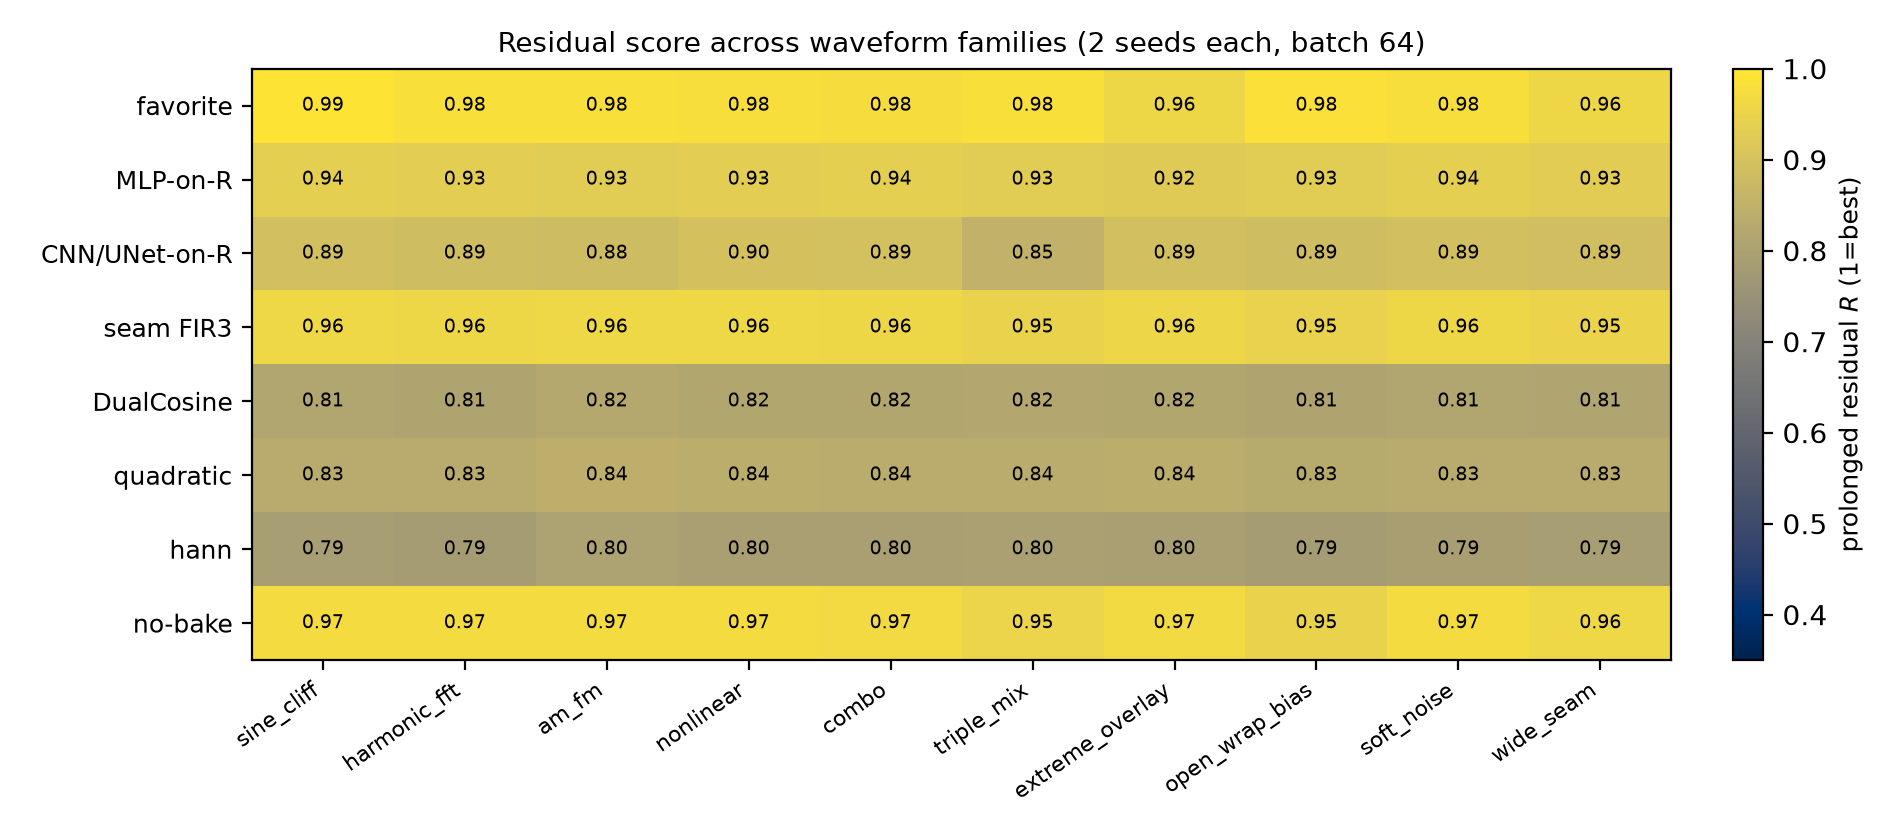
\includegraphics[width=\columnwidth]{figures/fig_sota_heatmap.png}
  \caption{Colorblind-safe (\texttt{cividis}) heatmap of mean prolonged $R$ for selected methods $\times$ generative families (2 seeds each). Higher is better.}
  \label{fig:sota-heatmap}
\end{figure}

\begin{figure}[t]
  \centering
  
\includegraphics[width=\columnwidth]{figures/fig_sota_method_bars.png}
  \caption{Multi-family mean prolonged $R$ by method (same $20$-waveform board as Table~\ref{tab:sota-main}).}
  \label{fig:sota-method-bars}
\end{figure}

\subsection{Hard cliffs expose classical fade failure}
\label{sec:cliff-strata}

Does high no-bake $R$ hide DualCosine failure on large wrap jumps?
Table~\ref{tab:cliff-strata} stratifies a $4{,}096$-tile holdout draw (seed \texttt{20260719}) by engine wrap-jump percentiles (p75$\approx 1.387$, p90$\approx 1.832$), frozen in the \href{https://github.com/reeldemo/denoise-opt-meta/blob/master/paper/Unsupervised_Wavetable_Seam_Artifact_Repair_via_Hybrid_GA-PPO_Meta-Search_v11/figures/cliff_strata.json}{cliff-strata data}.
This board uses whole-curve prolonged $R$ (historical, not $R_{\mathrm{blend}}$).
No-bake $R$ can stay high on mild cliffs because residual mass remains small relative to ideal RMS.
DualCosine collapses on hard cliffs ($0.819$ $\to$ $0.657$), while the meta favorite holds ($R\approx 0.9915$)
and corrupt$\to$corrupt N2N stays slightly ahead ($R\approx 0.9922$ on all / top-10\%).
Favorite wrap-jump on the top-10\% subset stays $\approx 1.83$ (vs no-bake $2.09$).
The claim is tiled residual repair, not endpoint-zeroing.
\textbf{Edge RMSE} is the locked required seam-local secondary (EVAL\_PROTOCOL): on the top-10\% subset it drops from no-bake $0.095$ to favorite $0.021$ (N2N corrupt$\to$corrupt also $0.021$, DualCosine $0.990$).
Click energy remains an optional diagnostic.

\begin{table*}[t]
  \centering
  \caption{Cliff strata on $4{,}096$ holdout tiles (historical prolonged $R$). Strata by engine wrap-jump.}
  \label{tab:cliff-strata}
  \setlength{\tabcolsep}{2.5pt}
  \begin{tabular}{@{}lrrrrrr@{}}
    \toprule
    Method & all $R$ & all jump & top25 $R$ & top25 jump & top10 $R$ & top10 jump \\
    \midrule
    seq LSTM (ceiling) & 0.9953 & 0.865 & 0.9955 & 1.637 & 0.9955 & 1.810 \\
    N2N sibling-sup. & 0.9936 & 0.879 & 0.9936 & 1.668 & 0.9934 & 1.842 \\
    N2N corrupt$\to$corrupt & 0.9922 & 0.870 & 0.9924 & 1.647 & 0.9922 & 1.821 \\
    neural favorite & 0.9911 & 0.869 & 0.9915 & 1.645 & 0.9915 & 1.825 \\
    seq CNN1D & 0.9863 & 0.881 & 0.9869 & 1.684 & 0.9867 & 1.871 \\
    no-bake & 0.9715 & 0.913 & 0.9713 & 1.797 & 0.9667 & 2.094 \\
    \texttt{seam\_fir3} & 0.9611 & 0.456 & 0.9461 & 0.893 & 0.9429 & 1.034 \\
    DualCosine & 0.8193 & 0.335 & 0.6864 & 0.290 & 0.6574 & 0.335 \\
    \bottomrule
  \end{tabular}\\[0.3em]
  {\footnotesize $n$: all $4096$, top25 $1024$, top10 $410$.}
\end{table*}

\begin{table}[t]
  \centering
  \caption{Required seam-local secondary on top-10\% wrap-jump tiles ($n{=}410$): edge RMSE (lower better). Frozen in the \href{https://github.com/reeldemo/denoise-opt-meta/blob/master/paper/Unsupervised_Wavetable_Seam_Artifact_Repair_via_Hybrid_GA-PPO_Meta-Search_v11/figures/cliff_strata.json}{cliff-strata data}.}
  \label{tab:cliff-edge-rmse}
  \setlength{\tabcolsep}{3pt}
  \begin{tabular}{@{}lr@{}}
    \toprule
    Method & top10 edge RMSE \\
    \midrule
    seq LSTM & 0.011 \\
    N2N sibling-sup. & 0.018 \\
    neural favorite & 0.021 \\
    N2N corrupt$\to$corrupt & 0.021 \\
    seq CNN1D & 0.035 \\
    no-bake & 0.095 \\
    \texttt{seam\_fir3} & 0.164 \\
    DualCosine & 0.990 \\
    \bottomrule
  \end{tabular}
\end{table}

\subsection{Noise2Noise and sequence baselines}
\label{sec:n2n-baselines}

How does DenoiseOpt compare to true Noise2Noise-style and lightweight seq restorers on the same generator?
Primary corrupt$\to$corrupt N2N (20k Adam steps, 53k params, train seed \texttt{424242}) reaches canonical $R\approx 0.9917$, matching the meta favorite within $\approx 0.001$.
Secondary sibling-supervised N2N reaches $R\approx 0.9933$.
A bidirectional LSTM (76k params, 15k steps, train seed \texttt{424243}) is the supervised ceiling at $R\approx 0.9952$.
A tiny depthwise 1D CNN (3.2k params) reaches $R\approx 0.9864$.
Holdout tiles never enter training.
Classical DualCosine / \texttt{seam\_fir3} remain in Table~\ref{tab:cliff-strata}.
Figure~\ref{fig:n2n-vs-ours} plots these canonical holdout scores beside no-bake, DualCosine, and the neural favorite.

\begin{figure}[t]
  \centering
  
\includegraphics[width=\columnwidth]{figures/fig_n2n_vs_ours_bars.png}
  \caption{Canonical holdout prolonged $R$: N2N and seq baselines vs Ours (neural favorite).
    Train seeds \texttt{424242}/\texttt{424243} are disjoint from holdout \texttt{20260719}.}
  \label{fig:n2n-vs-ours}
\end{figure}

\subsection{Factory exports and AKWF cycles}
\label{sec:real-wt}

Does the wrap protocol transfer beyond synthetic sine cliffs onto true exports and third-party OA cycles?
Table~\ref{tab:real-wt} scores ReelSynth-exported factory periods (primary realism, $n{=}25$, byte-true factory frames resampled to $L{=}256$) and Adventure Kid Waveforms (AKWF) CC0 single-cycle WAVs (secondary, $n{=}24$) after close-seam idealization and the same open-wrap cliff.
Procedural stand-ins are demoted to tertiary smoke and no longer carry the primary realism claim.
On exported factory periods the favorite ($R{\approx}0.911$) trails no-bake / \texttt{seam\_fir3} / poly while still beating Dual Cosine ($0.883$).
On AKWF OA cycles the favorite ($R{\approx}0.970$) matches no-bake and beats Dual Cosine ($0.936$).
Export gaps are listed in Section~\ref{sec:limitations}.

\begin{table}[t]
  \centering
  \caption{Wavetable-native wrap protocol. Close-seam ideal $\to$ open-wrap cliff (seed \texttt{20260719}). Mean prolonged $R$. Primary = ReelSynth export. Secondary = AKWF CC0 files.}
  \label{tab:real-wt}
  \setlength{\tabcolsep}{3pt}
  \begin{tabular}{@{}lrr@{}}
    \toprule
    Method & Export ($n{=}25$) & AKWF OA ($n{=}24$) \\
    \midrule
    endpoint-pin (mean) & 0.939 & 0.978 \\
    \texttt{seam\_fir3} & 0.971 & 0.975 \\
    poly seam ($d{=}3$) & 0.967 & 0.970 \\
    no-bake & 0.967 & 0.969 \\
    neural favorite & 0.911 & 0.970 \\
    DualCosine & 0.883 & 0.936 \\
    N2N corrupt$\to$corrupt & 0.869 & 0.974 \\
    seq CNN1D & 0.839 & 0.962 \\
    seq LSTM & 0.769 & 0.948 \\
    \bottomrule
  \end{tabular}
\end{table}

\subsection{Polynomial baseline and endpoint pinning}
\label{sec:poly-jump}

Does a cheap classical poly fitter close the residual, and does endpoint pinning show the wrap-jump vs $R$ tradeoff?
A seam-local degree-3 polynomial fitter (no learning) reaches canonical $R\approx 0.972$ ($\approx$ no-bake) with wrap-jump essentially unchanged (\href{https://github.com/reeldemo/denoise-opt-meta/blob/master/paper/Unsupervised_Wavetable_Seam_Artifact_Repair_via_Hybrid_GA-PPO_Meta-Search_v11/figures/poly_baseline.json}{polynomial results}).
SSM seq models are deferred. The LSTM remains the supervised seq ceiling.
An endpoint-pin control (\href{https://github.com/reeldemo/denoise-opt-meta/blob/master/paper/Unsupervised_Wavetable_Seam_Artifact_Repair_via_Hybrid_GA-PPO_Meta-Search_v11/figures/jump_control.json}{pinning results}) drives wrap-jump to $0$ on all / hard subsets while dropping $R$ (all $0.906$, hard $0.822$).
Methods that zero wrap-jump are not the same objective as prolonged $R$ (Limitations).

\subsection{Classical virtual-analog seam repairs}
\label{sec:va-seam-baselines}

Do the cited VA antialias tools~\cite{stilson1996,nam2009polyblep,esqueda2016blamp} beat DualCosine on prolonged $R$ when applied as cycle-local seam residuals?

\paragraph{What each operator changes.}
Figure~\ref{fig:va-seam-techniques} shows the family on one high-wrap sine{+}cliff tile (same seed and tile as Figure~\ref{fig:intro-sine}).
\textbf{BLIT/BLEP} (Stilson/Smith lineage) treats the wrap as a value step.
It subtracts a band-limited step residual (here a raised-cosine BLEP-family lobe scaled by the measured wrap jump) so the tiled click spectrum is softened near the seam.
\textbf{PolyBLEP} (Nam et al.) is a cheap polynomial surrogate of that step residual with fractional-delay support near phase wrap.
It edits only a few samples on each side of the discontinuity.
\textbf{BLAMP} (Esqueda et al.) corrects a slope or corner jump (discontinuity in the first derivative), which matters for triangles, rectification, and hard clipping.
On a pure value cliff the slope jump is small, so BLAMP is nearly a no-bake passthrough.
\textbf{DualCosine} (our classical bake baseline) fades both ends of the stored period with raised-cosine windows.
It does not insert a BLEP-style residual.
It trades wrap energy for a wide end-fade distortion that prolonged $R$ penalizes on hard cliffs.

\paragraph{Scores.}
Table~\ref{tab:va-seam-blep} reports batch means from the \href{https://github.com/reeldemo/denoise-opt-meta/blob/master/paper/Unsupervised_Wavetable_Seam_Artifact_Repair_via_Hybrid_GA-PPO_Meta-Search_v11/figures/va_seam_blep.json}{VA results} (seed \texttt{20260719}, batch 64).
Implementation is released in the \href{https://github.com/reeldemo/reelsynth}{ReelSynth repository}. PolyBLEP matches \texttt{osc::va::poly\_blep}. BLIT/BLEP uses a raised-cosine step residual. BLAMP applies a polyBLAMP lobe to the wrap slope jump.
PolyBLEP reaches mean $R\approx 0.929$ ($\Delta R\approx{+}0.104$ vs DualCosine) but trails no-bake / \texttt{seam\_fir3} / the meta favorite.
BLIT/BLEP nearly zeros wrap-jump ($0.004$) while dropping mean $R$ to $0.868$ and collapsing on hard cliffs ($R\approx 0.712$).
BLAMP is near-no-bake on this value-cliff geometry (mean $R\approx 0.972$).
On the annotated severe tile in Figure~\ref{fig:va-seam-techniques}, tile $R$ is lower still (PolyBLEP $\approx 0.869$, BLIT/BLEP $\approx 0.703$, DualCosine $\approx 0.603$, BLAMP $\approx$ engine), which matches the hard-cliff strata.
These classical tools are scored here, not only cited.
They beat DualCosine on mean $R$ in places.
None matches the favorite on prolonged $R$.

\begin{figure*}[t]
  \centering
  
\includegraphics[width=\textwidth]{figures/fig_va_seam_techniques.png}
  \caption{Classical VA seam techniques on one cracked sine{+}cliff tile (seed~\texttt{20260719}, tile~46, $|wrap|{=}2.283$, $L{=}256$, three tiled periods). Yellow band marks the first seam neighborhood. Panel tile $R$ (1~=~best): (a)~ideal (unscored sibling). (b)~cracked engine $R{=}0.9503$. (c)~BLIT/BLEP step residual $R{=}0.7026$. (d)~PolyBLEP fractional-delay residual $R{=}0.8685$. (e)~BLAMP slope/corner residual $R{=}0.9504$ (near no-bake on value cliffs). (f)~DualCosine end fade $R{=}0.6029$. Colorblind-safe hues with distinct linestyles for B\&W print. Batch means appear in Table~\ref{tab:va-seam-blep}. Accessibility: six-panel comparison of ideal, cracked, BLIT/BLEP, PolyBLEP, BLAMP, and DualCosine.}
  \label{fig:va-seam-techniques}
\end{figure*}

\begin{table*}[t]
  \centering
  \caption{Classical VA seam repairs on the residual protocol (seed \texttt{20260719}).
  Canonical holdout: $R$, SNR/SDR, wrap-jump, edge RMSE.
  Cliff top-10\%: $R$ ($n{=}410$).
  Multi: mean $R$ over 20 generative waveforms.}
  \label{tab:va-seam-blep}
  \setlength{\tabcolsep}{2.5pt}
  \begin{tabular}{@{}lrrrrrrr@{}}
    \toprule
    Method & $R$ & SNR & SDR & jump & edge & top10 $R$ & multi $R$ \\
    \midrule
    BLAMP & 0.9718 & 32.6 & 32.7 & 0.873 & 0.080 & 0.9667 & 0.965 \\
    no-bake & 0.9718 & 32.6 & 32.7 & 0.873 & 0.080 & 0.9667 & 0.965 \\
    \texttt{seam\_fir3} & 0.9610 & 29.6 & 29.6 & 0.438 & 0.112 & 0.9429 & 0.955 \\
    PolyBLEP & 0.9288 & 25.9 & 25.8 & 0.102 & 0.205 & 0.8641 & 0.924 \\
    BLIT/BLEP & 0.8680 & 20.4 & 20.3 & 0.004 & 0.365 & 0.7116 & 0.860 \\
    DualCosine & 0.8249 & 18.0 & 17.8 & 0.292 & 0.506 & 0.6574 & 0.814 \\
    \bottomrule
  \end{tabular}\\[0.3em]
  {\footnotesize Latency (canonical, CUDA): PolyBLEP $\approx 1.43$\,ms/batch, DualCosine $\approx 1.06$, BLIT/BLEP $\approx 123$, BLAMP $\approx 54$. Frozen in the \href{https://github.com/reeldemo/denoise-opt-meta/blob/master/paper/Unsupervised_Wavetable_Seam_Artifact_Repair_via_Hybrid_GA-PPO_Meta-Search_v11/figures/va_seam_blep.json}{VA results}.}
\end{table*}

\subsection{When search helps vs classical methods}
\label{sec:transfer}

Per-cycle $\Delta R$ on export, AKWF, Rust \texttt{sound\_bench}, and sine{+}cliff holdout
(\href{https://github.com/reeldemo/denoise-opt-meta/blob/master/paper/Unsupervised_Wavetable_Seam_Artifact_Repair_via_Hybrid_GA-PPO_Meta-Search_v11/figures/transfer_failures.json}{transfer results}):
favorite win-rate vs Dual Cosine is high on sine cliffs ($1.00$) and AKWF ($0.88$), and moderate on export ($0.64$) / Rust ($0.75$).
Win-rate vs no-bake is high only on sine cliffs ($0.92$) and collapses on export ($0.24$) / Rust ($0.20$).
Search value is highest on hard cliffs and when compact bake graphs are needed without engine$\to$ideal labels at search time.
Export / Rust gaps vs no-bake are listed in Section~\ref{sec:limitations}.

\subsection{Transfer to Rust engine tiles}
\label{sec:rust-bench}

Table~\ref{tab:rust-bench} scores the Python-trained favorite on 20 Rust-exported tiles.
The favorite beats Dual Cosine (mean $\Delta R{+}0.063$, Wilcoxon $p{\approx}0.009$) but trails no-bake and \texttt{seam\_fir3} on absolute $R$.
The primary SOTA claim remains the Python multi-family matrix.

\begin{table}[t]
  \centering
  \caption{Rust \texttt{sound\_bench} transfer ($n{=}20$). Prolonged $R$. $\Delta R$ vs Dual Cosine.}
  \label{tab:rust-bench}
  \setlength{\tabcolsep}{3pt}
  \begin{tabular}{@{}lrr@{}}
    \toprule
    Method & $R$ (20 Rust tiles) & $\Delta R$ vs Dual Cosine \\
    \midrule
    no-bake & $0.928\pm0.084$ & ${+}0.166$ \\
    \texttt{seam\_fir3} & $0.896\pm0.077$ & ${+}0.134$ \\
    neural favorite & $0.825\pm0.121$ & ${+}0.063$ \\
    classic quadratic & $0.788\pm0.110$ & ${+}0.026$ \\
    Dual Cosine / cosine fade & $0.762\pm0.118$ & $0$ \\
    \bottomrule
  \end{tabular}
\end{table}

\begin{figure}[t]
  \centering
  
\includegraphics[width=\columnwidth]{figures/fig_inference_vs_residual.png}
  \caption{High-$R$ fitted operators: residual vs CUDA latency. Star: favorite.}
  \label{fig:inference-pareto}
\end{figure}

\begin{figure}[t]
  \centering
  
\includegraphics[width=\columnwidth]{figures/fig_inference_latency_bars.png}
  \caption{Inference latency for high-$R$ fitted models (CUDA, batch 64).}
  \label{fig:inference-bars}
\end{figure}

\begin{figure}[t]
  \centering
  
\includegraphics[width=\columnwidth]{figures/fig_classical_vs_ai_scatter.png}
  \caption{Canonical holdout: classical methods and favorite in the $R$ vs ms/batch plane.}
  \label{fig:classical-vs-ai-scatter}
\end{figure}

\begin{figure}[t]
  \centering
  
\includegraphics[width=\columnwidth]{figures/fig_classical_vs_ai_bars.png}
  \caption{Canonical holdout ranking on prolonged $R$ (left) and latency (right).}
  \label{fig:classical-vs-ai-bars}
\end{figure}
